\part{CÁLCULO DIFERENCIAL}
\chapter{Preliminares.}	\label{preliminares}

	\section{Introducción histórica}
	
		El cálculo infinitesimal es la \emph{matemática del cambio}, tiene dos ramas principales: el cálculo diferencial y el cálculo integral. Ambos forman un poderoso instrumento para atacar múltiples problemas de la física, ingenieras y otras ciencias, incluidas las ciencias sociales.
	
		En sus inicios, s. XVII, el cálculo surgió al buscar la solución a dos problemas fundamentales inspirados por la física: el problema del trazado de rectas tangentes a una función en un punto, que permitirá la posibilidad de encontrar valores óptimos (máximos o mínimos) para estas funciones y que dará como resultado el cálculo diferencial y, el segundo problema, determinar la longitud de una curva, el área que hay bajo la misma y el cálculo de volúmenes, que dará lugar al cálculo integral. Quizás el descubrimiento más importante es que hay una conexión inesperada entre dos problemas clásicos aparentemente no relacionados: encontrar tangentes a una curva y calcular áreas. Lo veremos en el capítulo de la Integral Definida y le llamaremos \textit{Teorema Fundamental del Cálculo Integral }.
	
		Derivadas e integrales resolvían problemas que habían puesto a prueba el ingenio de matemáticos anteriores. Velocidades, tangentes, máximos y mónimos podan encontrarse utilizando diferenciación. Longitudes, áreas y volúmenes podan calcularse por integración. Parecía que las pautas de la naturaleza estaban escritas en el lenguaje del cálculo infinitesimal. 
	
		Fue ya en el s. XIX, con la construcción del cuerpo de los números reales, del concepto de función real y del concepto de límite, cuando se establecieron de manera rigurosa los fundamentos del cálculo. 

		%\vspace{5mm}
	
		\begin{figure}[H]
			\centering
			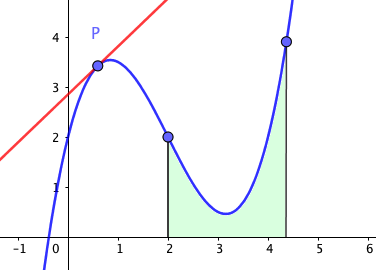
\includegraphics[width=0.5\textwidth]{imagenes/imagenes01/T01IM01.png}
			\caption{Los dos problemas clásicos del cálculo: trazado de tangentes y áreas bajo curvas.}
		\end{figure}
		
		Hemos visto como surgió el cálculo. Pero ?`\emph{qué es realmente el cálculo infinitesimal}?: El cálculo suele dividirse en dos partes, denominadas cálculo diferencial y cálculo integral. El cálculo diferencial investiga las propiedades de las razones de cambio de variables que están vinculadas por medio de ecuaciones. Por ejemplo, un resultado fundamental del cálculo diferencial es que si $y = x^n$, entonces la razón de cambio de $y$ con respecto a $x$ es $n x^{n-1}$. Resulta que cuando se usa la intuición para pensar en ciertos fenómenos (movimiento de los cuerpos, cambios en la temperatura, crecimiento de poblaciones y muchos otros), se llega a postular ciertas relaciones entre estas variables y sus razones de cambio. Estas relaciones se escriben en una forma conocida como ecuaciones diferenciales. Así, el objetivo principal de estudiar cálculo diferencial consiste en comprender qué son las razones de cambio y cómo escribir ecuaciones diferenciales. El cálculo integral proporciona métodos para recuperar las variables originales conociendo sus razones de cambio. La técnica para hacer esto se denomina integración, y el objetivo fundamental del estudio del cálculo integral es aprender a resolver las ecuaciones diferenciales proporcionadas por el cálculo diferencial.
	
	
	
	\section{ Axiomas, definiciones, teoremas $\; \divideontimes$}
	
	Para entender bien este apartado, el/la lector/a interesaso/a puede consultar el apéndice \ref{ap:logica} de `Intoducción a la lógica'. 
	
Suele decirse que en matemáticas no hay nada más que	axiomas y teoremas (bueno, también hay conjeturas, proposiciones, definiciones,...). Todo lo que se demuestra es un teorema, por ello el nombre teorema se reserva para resultados que se consideran realmente importantes y que ha costado esfuerzo llegar a probarlos. Se usan también los términos: corolario, lema, proposición, definición y otros. Pero la estructura de una teoría matemática  se resume en un conjunto de axiomas y de teoremas que se deducen de ellos mediante reglas de inferencia lógica. Veamos que es cada una de estas estructuras lógicas de las matemáticas.
	
		AXIOMA: enunciado cuya veracidad es admitida por todos/as y no necesita demostración.
	
		DEFINICIÓN: los objetos matemáticos existen mediante definiciones. Por ejemplo, un número puede ser natural y se llama número compuesto o número primo, par o impar, siempre que cumpla condiciones precisas y específicas. Estas condiciones son la definición del concepto.
	
		PROPOSICIÓN: enunciado cuya veracidad se ha demostrado.
	
		LEMA: proposición que es preciso demostrar antes de demostrar un teorema para que la demostración de este último no sea excesivamente larga.
	
		TEOREMA: enunciado en el que, a partir de una suposiciones iniciales (HIPÓTESIS) se consigue demostrar otro enunciado (TESIS).
	
		COROLARIO: son teoremas consecuencia inmediata de otro teorema anterior al que se le considera de mayor importancia.
		
		 Un teorema escrito en la forma H (hipótesis)$\; \to\; $ T (Tesis), se llama \emph{teorema directo} y se lee "si se verifica H, entonces se verificará T". Hay otros teoremas relacionados con el directo:
		
		\emph{Teorema contrario:} no H $\; \to\; $ no T
		
		\emph{Teorema recíproco:} T $\; \to\; $ H
		
		\emph{Teorema contrarrecíproco:} no T $\; \to\; $ no H
		
		Ejemplos:
		
		\hspace{10mm} Directo: Ser madrileño (H) implica ser español (T)
		
		\hspace{10mm} Recíproco: Ser español (T) implica ser madrileño (H): No se verifica, ser español no implica ser madrileño.
		
		\hspace{10mm} Contrario: no ser madrileño (no H) implica no ser español (no T): No se verifica, se puede ser español sin ser madrileño, p.e., siendo andaluz.
		
		\hspace{10mm} Contrarrecíproco: no ser español (no T) implica no ser madrileño (no H): Sí se verifica, si no eres español no puedes ser madrileño.
			
		\vspace{4mm} CONDICIONES NECESARIAS Y SUFICIENTES: 
		
		$M \to A \quad$: A es \emph{condición necesaria} para que se cumpla M. Ejemplo: M="ganar la liga de fútbol de primera división", A="jugar en primera división"	
		
		$B \to M \quad$: B es \emph{condición suficiente} para que se cumpla M. Ejemplo: M="ganar la liga de fútbol de primera división", B="ser el equipo con más puntos al finalizar la liga".
		
		$C \longleftrightarrow  M \quad$:  C es \emph{condición necesaria y suficiente} de M. Ejemplo: M="ganar la liga de fútbol de primera división", C="recibir el trofeo de campeón al finalizar la liga".
		
		
		\vspace{4mm} \emph{Nota:} Cuando acaba la demostración de un teorema es usual advertírselo al lector por si ha de volver a empezar a releer la misma. Para ello se suele escribir cosas como ``c.q.d'', como queramos demostrar; ``q.e.d'', quod erat demonstrandum (en latín) y, la que usaremos nosotros, que será el símbolo $\Box$ situado al final y a la derecha de la última línea de la demostración.
		
		

	\section{Los números reales}
	
	El hombre ha necesitado, a través de su historia, de los números naturales para contar, de los enteros para el comercio, de los racionales para sus construcciones. Ya los griegos (escuela pitagórica) se dieron cuenta de que existían otro tipo de números extraños a los que llamaron irracionales, lo que nos lleva a nuestro objetivo de los números reales, base del cálculo.
	
		Números naturales $\mathbb N$: 1, 2, 3, ...
	
		Números enteros $\mathbb Z$: ... , -2, -1, 0, 1, 2, 3, ...
	
		Números racionales $ \mathbb {Q} =\left\{\dfrac p q; \  p,q\in \mathbb {Z}; \ q>0; \ mcd\ (p,q)=1 \right\}$. Es decir, son el conjunto de las fracciones irreducibles de números enteros con denominador positivo (no nulo). Sabemos que su expresión decimal siempre es un número entero, decimal exacto o decimal periódico y sabemos pasar de escritura decimal (en estos casos) a escritura en forma de fracción y viceversa. 
		
		Pero hay números cuya expresión decimal es infinita y no periódica, luego no se pueden expresar como fracción ($\sqrt 2$ no es racional, lo veremos más adelante, en el apartado dedicado a la demostración por \emph{reducción al absurdo}) (sección \ref{reduc-absurd}). Este nuevo tipo de números son los IRRACIONALES ($\pi, \ e, \ \sqrt[3]{5}, \ ..$)
	
		Número reales $\mathbb R$: es el conjunto formado por todos los números racionales e irracionales.
	
		Dados $x,y \in \mathbb R$, representaremos por $x+y$ la suma de números reales y por $xy$ el producto.
	
		
	
	\subsection{Axiomas algebraicos}
		
		\begin{axio}[Axiomas Algebraicos] Responden de las propiedades de la suma y producto de números reales. Son los siguientes:	
		\end{axio}
 
	
		\begin{itemize}
		\item ASOCIATIVAS:  
			\begin{equation}
			\forall x,y,z  \in  \mathbb R: \quad
			(x+y)+z=x+(y+z);  \qquad (xy)z=x(yz)
			\end{equation}
	
		\item CONMUTATIVAS:  
			\begin{equation}
			\forall x,y  \in  \mathbb R: \quad
			x+y=y+x;  \qquad xy=yx
			\end{equation}
	
		\item ELEMENTOS NEUTROS:  Hay dos números reales \textit{distintos} $0$ y $1$ tales que $\forall x \in \mathbb R$ se verifica:
			\begin{equation}
		    0+x=x;  \qquad 1x=x
			\end{equation}
	
		\item ELEMENTOS OPUESTO E INVERSO:  Para cada número real $x$ hay un número real llamado \textit{opuesto} de x, que representamos por $-x$ tal que: 
			\begin{equation}
			x+(-x)=0
			\end{equation}
			Para cada número real $x$ distinto de cero, $x \neq 0$, hay un número real llamado \textit{inverso} que representamos por $x^{-1}$, tal que  
			\begin{equation}
			xx^{-1}=1
			\end{equation}
		\item DISTRIBUTIVA:  
			\begin{equation}
			\forall x,y,z  \in  \mathbb R: \quad
			(x+y)z=xz+yz
			\end{equation}
		\end{itemize}
	
		
	
		\begin{prop}
		Se verifican las siguientes igualdades:	
		\begin{equation}
		0x=0; \qquad (-x)y=-xy; \qquad (-x)(-y)=xy
		\end{equation}
		\end{prop}
	
		\begin{proof}
		
	 	Probaremos primero que 0x = 0. Por la propiedad distributiva:$(0 + 0)x = 0 x + 0 x$ . 
	 	
	 	
	 	Como consecuencia del elemento neutro es $0 + 0 = 0$. Obtenemos as que $0x=0x+0x$.
	 	Teniendo en cuenta el elemento neutro de la suma:  $0 x = 0$.
	 	Probaremos ahora que $(-x)y =  - (xy)$. Tenemos que $xy + (-x)y = (x + (-x))y = 0 y = 0$. Donde hemos usado el opuesto, la distributiva y el apartado anterior. 
		
		La igualdad $xy + (-x)y = 0$ nos dice, por el elemento opuesto, que $(-x)y$ es el opuesto de $xy$. Eso es justamente lo que queramos probar

		Finalmente, la igualdad $(-x)(-y) = xy$ es consecuencia inmediata de la anterior.
	
		\end{proof}

		El símbolo $-x$ debe leerse siempre el opuesto de $x$ y no menos $x$. La razón es que la palabra menos  remite a una idea de orden (si hay menos  es porque hay más ) y el significado de $-x$ es puramente algebraico y nada tiene que ver con la idea de orden de la que ni siquiera hemos hablado  !`No cometas el error de pensar que $-x$ es negativo!

		Notación. Suele escribirse $x - y$ en vez de $x + (-y)$. También, supuesto $y \neq 0$, se escribe $x/y$ o $\frac x y$ en vez de $xy^{-1}$.
	
		
	
	\subsection{Axiomas de orden}
		
		\begin{axio}[Axiomas de orden]
			La ordenación de números reales establece que su representación en una recta consiste en fijar un punto, \textit{origen}, donde se coloca el $0$ y los números situados a su derecha son los \textit{positivos}, representados por $\mathbb R^+$. Las propiedades del orden son:
		\end{axio}
		
		\begin{itemize}
		\item LEY DE TRICOTOMÍA. Para cada número real $x$ se verifica una sola de las tres siguientes afirmaciones:  $x=0$, $x$ es positivo, $-x$ es positivo.
		\item ESTABILIDAD DE $\mathbb R^+$. La suma y producto de números positivos también es un número positivo.
		\item RELACIÓN DE ORDEN. La ley de Tricotomía en particular dice que el $0$ no es positivo. Por otra parte, como $x+(-x)=0$, por la ley de estabilidad de $\mathbb R^+$ concluimos que $-x$ no es positivo. Los elementos del conjunto $\mathbb R^- = \{ -x: x\in \mathbb R^+ \} $ se llaman \textit{números negativos} y son los opuestos a los números positivos.
		\end{itemize}
	
		
		
		\begin{defi} Para $\;x,y  \in \mathbb R\;$, escribimos $\;x<y\;$ o $\; y>x\; $ para indicar que $\; y-x \in \mathbb R^+\; $ y escribimos $\; x\le y$ o $y \ge x\; $ para indicar $\; y-x \in \mathbb R^+ \cup \{ 0 \} = \mathbb R^+_0\; $(Notación: $\; \mathbb R^-_0=\mathbb R^-\cup \{ 0 \};\; \mathbb R^*=\mathbb R \sim \{ 0 \}\; $)
		\end{defi}
		
	
		\begin{prop}
		Para todo $x\neq 0$ se verifica que $x^2>0$. En particular, $1>0$.
		\end{prop}
	
		\begin{proof}
		Si $\;x\neq 0 \;$, por la ley de tricotomía o bien $x$ es positivo o bien $-x$ es positivo. Como $\; x^2=xx=(-x)(-x)\; $, concluimos que $x^2$ es positivo, nos apoyamos en la ley de estabilidad del producto en $\mathbb R^+$, ambas leyes de los axiomas de orden de los números reales.. En particular tenemos que $1^2=1>0$. !`El $1$ es positivo! 
		\end{proof}
		
		
	\subsection{Propiedades topológicas de los números reales}
	 
	 Daremos, sin demostración, las siguientes propiedades de los números reales:
	 
	
	\begin{enumerate}[Prop.R.1]
	
		\item $\mathbb R$ es \emph{arquimediano}: $\forall x \in \mathbb R \; \; \exists n \in \mathbb N \; : \; x<n$
		\item $\forall x \in \mathbb R \; \forall y \in \mathbb R^{+} \;  \exists n \in \mathbb N \: : \; x<ny $. Geométricamente significa que todo segmento ($x$), por grande que sea, se puede recubrir con unidades tan pequeñas como se quiera ($y$). De otro modo, con una regla, por pequeña que sea, se puede cubrir cualquier distancia (basta colocarla sucesivamente las veces que haga falta).
		\item $\mathbb R\; $es \emph{denso}: 
		
		$a)\quad \forall x,y \in \mathbb R$ con $x<y,\;\; \exists q \in \mathbb Q:\; \; x<q<y$
		
		$b)\quad \forall x,y \in \mathbb R$ con $x<y,\;\; \exists \alpha  \in \mathbb R \sim \mathbb Q: \; \; x<\alpha<y$
		
		 
	\end{enumerate}
	
	\subsection{Desigualdades}
	 Las desigualdades son un tema muy importante que hay que aprender a manejar correctamente mediante la práctica de muchos ejemplos y ejercicios. Siempre hay que respetar las reglas generales que las gobiernan y se dan en el siguiente teorema.	
			
		\begin{teor}[Reglas para trabajar con desigualdades.] 	
		Sean $x,y,z \in \mathbb R$ 
		\end{teor}
		\begin{enumerate}
			\item $x \le y \;$ e $\; y\le z\; $ implican que $\; x\le z$
			\item $x \le y \;$ e $\; y\le x\; $ implican que $\; x=y$
			\item Se verifica exactamente una de las tres relaciones: $\; x<y\; $, $\; x=y \; $ o $\; y<x$
			\item $x<y\; $ implica que $\; x+z<y+z\; $
			\item $x<y,\; z>0$ implican que $\; xz<yz$
			\item $x<y,\; z<0$ implican que $\; xz>yz$
			\item $xy>0\;$ sí, y solo si, $x$ e $y$ son los dos positivos o los dos negativos. En consecuencia, si $x\neq 0$, entonces $\; x^2>0\; $ y, en particular, $1>0$
			\item $z>0\;$ implica que $\; \frac 1 z >0$
			\item supuestos $x$ e $y$ ambos positivos o ambos negativos, se cumple que $\; x<y \; $ implica $\; \frac 1 y < \frac 1 x \;$
		\end{enumerate}
	
		\begin{proof}
			Todas estas propiedades son fáciles de probar. P.e., el apartado 5, si $x<y$ se tiene que $y-x>0$. Tomando $z>0$, también será $z(y-x)>0$, es decir, $zy-zx>0$, o sea $zx<zy$. Lo único que hay que tener en cuenta para demostrar todos los apartados de este teorema son las definiciones de los símbolos $<$ y $>$ y los axiomas algebraicos y de orden de los números reales. El resto de la demostración se deja como ejercicio.
		\end{proof}
		
		
	\subsection{Ínfimo y Supremo. Axioma de completitud $ \; \divideontimes$}
	
	Antes de enunciar el último axioma de los números reales, veamos las siguientes definiciones:
	
		\begin{defi} Sea $A \subset \mathbb R$, entonces
		
			\begin{itemize}
				\item [*] Si existe $x \in \mathbb R$ tal que $x>a$ para todo $a \in A$, entonces $x$ se llama 'cota superior' de A y se dice que el conjunto $A$ está 'acotado superiormente'.
				\item [*] Si existe $x \in \mathbb R$ tal que $x<a$ para todo $a \in A$, entonces $x$ se llama 'cota inferior' de A y se dice que el conjunto $A$ está 'acotado inferiormente'.
			\end{itemize}
		
		\end{defi}
		
		\begin{defi}
		Sea $A \subseteq  \mathbb R$ acotado superiormente y supongamos que existe un $a\in \mathbb R$ que satisface las siguientes dos condiciones:
		
			\begin{itemize}
				\item [---] $a$ es una cota superior de $A$
				\item [---] si $b\in \mathbb R$ es cota superior de $A$, entonces $a\le b$
			\end{itemize}
			
		Entonces $a$ es el 'supremo' de A, es 'la menor de las cotas superiores"
		\end{defi}

		\begin{defi}
		Sea $A \subseteq \mathbb R$ acotado inferiormente y supongamos que existe un $a\in \mathbb R$ que satisface las siguientes dos condiciones:
		
			\begin{itemize}
				\item [---] $a$ es una cota inferior de $A$
				\item [---] si $c\in \mathbb R$ es cota inferior de $A$, entonces $a\ge c$
			\end{itemize}
			
		Entonces $a$ es el 'ínfimo' de A, es 'la mayor de las cotas inferiores"
		\end{defi}
		
		\begin{axio}Axioma de completitud.
		
			\begin{itemize}
				\item [---] Todo conjunto no vacío de números reales acotado superiormente tiene supremo-
				\item [---] Todo conjunto no vacío de números reales acotado inferiormente tiene ínfimo.
			\end{itemize}
			
		\end{axio}

	
		\begin{defi} Se dice que un conjunto no vacío de números reales $A \subset \mathbb R$, tiene \emph{máximo} si hay un número $M\in A$ que es el mayor de todos los elementos de A, es decir, $x\le M,\; \forall x \in A$. En este caso escribimos $M=max\, A$. Si $\exists m \in A : m\le x;\, \forall x \in A$, m es el \emph{mínimo} de A, $m=min\, A$.
		
			De otro modo, si el supremo de $A$ está en $A$, se le llama máximo. Si el ínfimo de $A$ está en $A$, se le llama mínimo.
		\end{defi}
		
		
	
	
	\subsection{Valor absoluto}
	
	\begin{defi}[Valor Absoluto.] El valor absoluto de un número real $\, x\in \mathbb R\, $ se define como el número:
	\begin{equation}
		|x|=
		\begin{cases} 
		\;\;  x &\mbox{ si } x\ge 0 \\ 
		\; -x & \mbox{ si } x<0 
		\end{cases}
	\end{equation}	
	\end{defi}
		El valor absoluto es, en matemáticas el \textit{gran positivizador}, $|3|=3;\quad |-2|=2; \quad |0|=0$.
	
	\begin{defi}
	Para cada $\; x\in \mathbb R^+_0\; $, representamos	por $\; \sqrt x\; $ al único número \emph{mayor o igual que cero} cuyo cuadrado es igual a $x$.
	\end{defi}
	En consecuencia, $\; \sqrt {x^2}=|x|\; $ (En efecto, $\;|x|^2=x^2 \; $ y, además, $\;|x| \ge 0 \; $, por tanto: $\; \sqrt {x^2}=|x|\; $)
	
	\begin{teor}[Propiedades del valor absoluto.] 	
	\end{teor}
		\begin{enumerate}
		\item $|-x|=|x|$
		\item $|xy|=|x|\cdot|y|$
		\item $\left| \dfrac x y \right| = \dfrac {|x|}{|y|}$
		\item $|x|\le y\;  \mbox{ es equivalente a } -y\le x \le y $
		\item $|x+y|\le|x|+|y|\qquad$ \emph{\underline{Desigualdad Triangular}}
		\item $\left|\,  {|x|-|y|}\,  \right| \le|x-y|\qquad$ La igualdad se da solo si $xy\ge 0$ 
	\end{enumerate}
	
	\begin{proof}
		Usaremos la estrategia siguiente: a) Para probar que dos números positivos son iguales es suficiente probar que sus cuadrados son iguales; y b) Para probar una desigualdad entre dos números positivos es suficiente con probar esa desigualdad para sus cuadrados.
		Para probar 1, 2, y 3, pe. la 2, tenemos que: 
		
		$|xy|^2=(xy)^2=x^2y^2=|x|^2 |y|^2=\left( |x||y|\right)^2 $
		
		\vspace{2mm}\hspace{-7mm}
		Para la desigualdad triangular:
		
		$|x+y|^2=(x+y)^2=x^2+2xy+y^2=|x|^2+2xy+|y|^2\le $
		$|x|^2+2|xy|+|y|^2= \left( |x|+|y| \right)^2$
		
		\vspace{2mm}\hspace{-7mm}
		La última propiedad: $||x||-|y||^2=x^2-2|x||y|+y^2\le $
		$ x^2 - 2 x y +y^2=(x-y)^2=|x-y|^2 \qquad$ La igualdad se verifica si, y solo si, $xy=|xy|$, es decir, $xy\ge 0$
		\end{proof}
		
		
		
		\begin{proof}[Otra forma de demostar la desigualdad triangular: $|x+y|\le|x|+|y|\;$ ].
		
		
		 Consideraremos 4 casos:
			 i) $x\ge0;\;\;y\ge0;\; \; $
			 ii) $x\ge0;\;\;y\le0;\; \; $
			 iii) $x\le0;\;\;y\ge0;\; \; $
			 iv) $x\le0;\;\;y\le0$	
			
			
			En el caso i) se verifica también que $x+y\ge0\;$ y, obviamente: $|x+y|=x+y=|x|+|y|$. En este caso se verifica la igualdad.
			
			En el caso iv), tenemos que $x+y\le 0$ y nuevamente se verifica la igualdad: $|x+y|=-(x+y)=-x+(-y)=|x|+|y|$
			
			 En el caso ii), cuando $x\ge 0\; $ y $\; y\le0$ , debemos probar que $|x+y|\le x - y$. este caso lo subdividiremos en dos subcasos:
			
			\hspace{10mm}$\diamond$  Si $x+y\ge 0$, tendremos que demostrar que $x+y\le x-y$; es decir, $y\le -y$. lo cual es cierto ya que $y\le 0$ y por tanto $-y\ge 0$
			
			\hspace{10mm}$\diamond$ Si $x+y\le 0$, debemos demostrar que $-x-y\le x-y$, es decir, $-x\le x$, lo cual es cierto ya que $x\ge 0$ y por tanto $-x\le 0$
			
			 Finalmente, el caso iii) puede demostrarse intercambiando $x$ por $y$ en la propiedad anterior. 
		\end{proof}
		
		\begin{proof}[Una tercera demostración de la desigualdad triangular] Haciendo uso se las propiedades del valor absoluto:
		
		$-|x|\le x\le |x|;\quad -|y|\le y\le |y|\quad $ Sumando ambas expresiones:
		
		$-\left( |x|+|y| \right) \le x+y \le \left( |x|+|y| \right)\quad $	Lo cual implica que: $|x+y|\le |x|+|y|$
			
		\end{proof}
		
		 Una figura como demostración sin palabras.
		
		
		\begin{figure}[H]
			\centering
			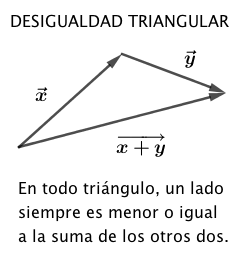
\includegraphics[width=0.4\textwidth]{imagenes/imagenes01/T01IM02.png}
			\caption {Desigualdad triangular: el módulo del vector suma de otros dos siempre es menor o igual a la suma de los módulos de los vectores sumados.}
		\end{figure}
		
		 \begin{defi} Llamamos \emph{distancia} entre dos números $x,y:\quad$ $\forall x,y \in \mathbb R:\; \; d(x,y)=|y-x|$
		\end{defi}
		
		 Se cumplen las siguientes propiedades para las distancias. La demostración se deja como ejercicio, se trata de aplicar las propiedades del valor absoluto.
		
		\begin{enumerate}[PD.1]
			\item  $\forall x \in \mathbb R:\; d(x,x)=0 $
			\item  $\forall x, y \in \mathbb R:\; d(x,y)=d(y,x)$
			\item  $\forall x, y, z \in \mathbb R:\; d(x,z) \le d(x,y)+d(y,z)$
		\end{enumerate}
		
		


		
	
	\subsection{Intervalos}
	
	\begin{defi} Es subconjunto de $I \subset \mathbb R$ tal que $\forall u,w \in I\; $, con $u\neq w\; $, y $\forall v \in \mathbb R\; $ con $u<v<w\; $ se cumpla que $v\in I$. Los intervalos pueden ser abiertos, cerrados y semiabiertos.\end{defi}
	
		\begin{figure}[H]
			\centering
			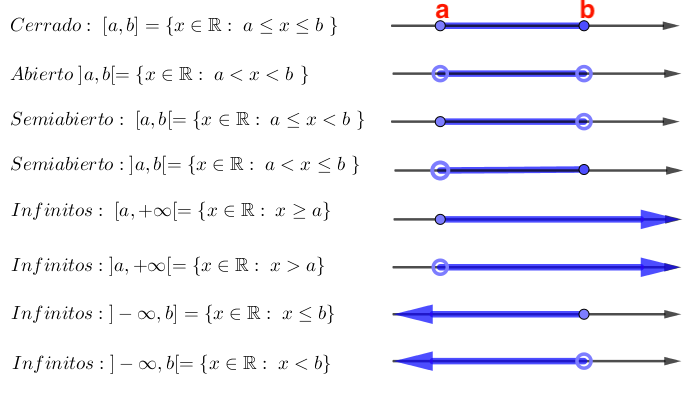
\includegraphics[width=0.7\textwidth]{imagenes/imagenes01/T01IM03.png}
		\end{figure}
		
		
		\begin{defi}[Entorno]: $\forall a \in \mathbb R, \; \forall r \in \mathbb R^{+}: $
		
		Se define el \emph{entorno} de centro $a$ y radio $r$ como todos los números reales cuya distancia a $a$ sea menor que $r$:
		
		$\quad E_r(a)=\{ \forall x \in \mathbb R \;  / \; d(a,x)<r \}=]a-r,a+r[$
		
		Se define el \emph{entorno reducido} de centro $a$ y radio $r$ como todos los números reales cuya distancia a $a$ sea menor que $r$, excluyendo al número $a$:
		
		$\quad E^*_r(a)=\{ \forall x \in \mathbb R \;  / \; 0<d(a,x)<r \}=]a-r,a+r[\sim \{a\}$
			
		\end{defi}
		
		\textbf{Valores Absolutos e Intervalos.}
		\begin{multicols}{2}
		\begin{itemize}
			\item $|x|=k \longleftrightarrow x=\pm k$
			\item $|x|<k \longleftrightarrow -k<x<k \longleftrightarrow ]-k,k[$
			\item $|x|\le k \longleftrightarrow -k\le x\le k \longleftrightarrow [-k,k]$
			\item $|x|> k \longleftrightarrow x>k\quad o \quad x<-k$
			\item $|x|\ge  k \longleftrightarrow x\ge k\quad o \quad x\le -k$
		\end{itemize}
		\begin{figure}[H]
			\centering
			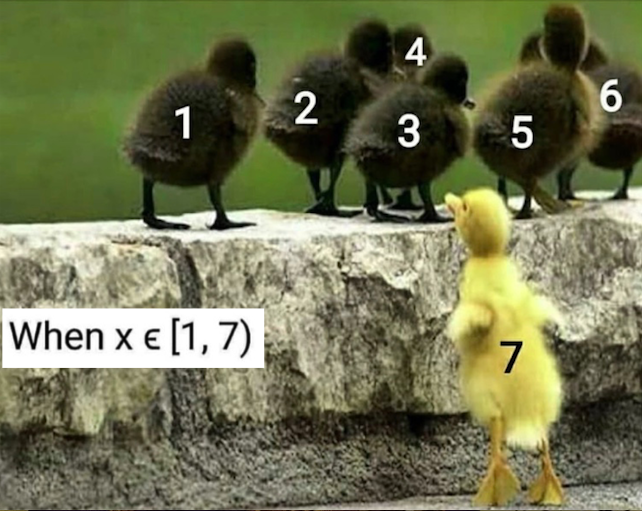
\includegraphics[width=0.4\textwidth]{imagenes/imagenes01/xiste01.png}
		\end{figure}
		\end{multicols}
		
		Recordando lo visto en la sección de supremo e ínfimo, en el intervalo $[2,5[, 2$ es el mínimo y $5$ el supremo.Además, como $2 \in [2,5[$, el intervalo tiene mínimo y éste es igual a $2$. Sin embargo, como $5 \notin [2,5[$ , el intervalo no tiene máximo
		
		\section{ Demostraciones en matemáticas $\; \divideontimes$} \label{demostraciones}
		
		\subsection{Principio de inducción matemática}
		\label{subsec:inducción}
		
		El \emph{Principio de inducción matemática} es un método de demostración que se usa para probar que ciertas propiedades matemáticas se verifican para todo número natural. Por ejemplo:
		$1^2+2^2+3^2+...+n^2=\frac 1 6 n (n+1)(2n+1)$
		
		Podemos comprobar fácilmente que se cumple esta relación para los valores $n$ concretos que se nos ocurra, pero queremos \emph{demostrar} que la relación es válida $\forall n\in \mathbb N$ y para ello usaremos el \emph{Principio de inducción matemática}, que podemos considerar como un axioma y lo entenderemos as:
		
		\begin{axio}[Principio de inducción matemática] Queremos probar que la propiedad $P(n)$ se verifica $\forall n\in \mathbb N$. Tendremos que seguir dos pasos:
			\begin{enumerate}
				\item Comprobaremos que el número 1 cumple la propiedad, es decir, $P(1)$ es cierta.
				\item Comprobaremos que si un número $n$ cumple la propiedad, \emph{entonces} también la satisface el número $n+1$. Es decir, si comprobamos que $P(n)$ es cierta, \emph{entonces} también lo es $P(n+1)$
			\end{enumerate}
			
			"Si tengo una escalera infinita y quiero poder llegar a cualquier peldaño, necesito dos cosas: un primer escalón y saber cómo dar un paso"
		\end{axio}

		
		\begin{ejem} \label{sum-cuad-induc}
		Probar que $\forall n\in \mathbb N$, se cumple:
		$1^2+2^2+3^2+...+n^2=\frac 1 6 n (n+1)(2n+1)$	
		\end{ejem}
		 Evidentemente, para $n=1$ se cumple: $1=1$
		
		\begin{proof}[Apliquemos el método de inducción.]
			
		Supongamos ahora que la propiedad es cierta para $n$, hemos de conseguir demostrar que también lo ha de ser para $n+1$, es decir, se ha de cumplir la propiedad cambiando la $n$ por $n+1$:
		
		$1^2+2^2+3^2+...+n^2+(n+1)^2=\frac 1 6 (n+1) (n+2)(2(n+1)+1)$ (*)
		
		Vamos a por ello, sumemos $(n+1)^2$ a ambos lados de la ecuación que suponemos válida para $n$:
		
		
		$1^2+2^2+3^2+...+n^2\; \; +(n+1)^2=\frac 1 6 n (n+1)(2n+1)\; \; +(n+1)^2=$
		(sacando $n+1$ factor común:)
		$=(n+1) \left( \frac 1 6 n (2n+1) +(n+1) \right)=$
		
		$=(n+1)\frac 1 6 \left(  n (2n+1) + 6(n+1) \right)=$
		$\frac 1 6 (n+1) (2n^2+7n+6)=$
		
		$=\frac 1 6 (n+1) (n+2) (2n+3)\; $ que es la expresión (*) que queramos demostrar.%$\Box$
		\end{proof}
		
		 
		Es necesario subrayar la importancia de la demostración de las dos partes del principio de inducción. Veamos un ejemplo de la importancia de la primera parte:
		
		\begin{ejem}
			Todo número natural es igual al número natural siguiente.
		\end{ejem}
		
		\begin{proof}[Mala aplicación del principio de inducción.]
			
		Aplicando la parte 2 del principio de inducción, resulta que si esto es cierto para $n$, es decir, $n=n+1$, basta con sumar $1$ a cada parte de la igualdad y escribir $n+1=n+1+1=n+2$, también será cierto para $n+1$.
		
		Obviamente la demostración no está acabada y el teorema es falso, pues falta comprobar la primera parte del método de inducción: la propiedad se cumple para $n=1$: falso, $1\neq 2$ %$\qquad \qquad \qquad \qquad \Box$
		\end{proof}
		
		Vamos a ver unos ejemplos a continuación que nos convenzan de la importancia de no quedarse con una conjetura encontrada sino que hay que demostrarla siempre.
		
		\begin{ejem}
			Sea $p(x)=x^4+x+41$, trinomio estudiado ya por Euler. Se tiene que $p(0)=41$, primo; $p(1)=43$, primo, y hasta $x=10$ se obtienen los números 47, 53, 61, 71, 83, 97, 113, 131 y 151 respectivamente, todos primos. Estaríamos tentados a afirmar que en este trinomio, al sustituir $x$ por cualquier número natural se obtiene un número primo, pero no es así, ya que, p.e., para $x=40$ tenemos $p(40)=40^2+40+41=40(40+1)+41=40\cdot 41+41=(40+1)\cdot 41=41^2$, que evidentemente no es un número primo.
		\end{ejem}
		
		 \begin{ejem} Consideremos los números de la forma $N(n)=2^{2^n}+1$. Para $n=0,1,2,3,4$ se obtienen $3, 5, 17, 257, 65537$, que son números primos. Fermat (s.XVII) aceptaba que todos los números obtenidos por esta fórmula eran primos. Fue Euler (s. XVIII) encontró $N(5)=4294967297=641\cdot 6700417$, compuesto.
		\end{ejem}
		
		\begin{ejem}
 			Leibniz (s. XVII) demostró que para cualquier número natural $n$, el número $n^3-n$ es siempre divisible por $3$, el número $n^5-n$ divisible por $5$, $n^7-n$ divisible por $7$. De ahí, supuso que si $k$ era un número natural impar, $n^k-n$ seria divisible por $k$, pero pronto observó que $2^9-2=510$ que no es divisible por $9$.
 		\end{ejem}
 		
 	    \begin{ejem}
 			$F(n)=991n^2+1$ no da nunca un cuadrado perfecto para $n=1,2,3,...$, por muchos das o años que nos dediquemos a ello. En efecto, el primer número natural para el que $F(n)$ resulta un cuadrado perfecto es:
 			
 			$n=12055735790331359447442538767.$
 		\end{ejem}
 		
 		 Con estos ejemplos podemos llegar a una sencilla pero importante conclusión: una conjetura puede ser cierta en muchos casos particulares pero si no hay demostración, nunca será un teorema.
		
		
		\subsection{Reducción al absurdo}
		\label{reduc-absurd}
		
		\begin{axio}[Reducción al absurdo]Una estrategia muy útil para demostrar que algo es cierto es suponer que es falso y llegar a una contradicción, el error habrá sido suponer que lo que queramos demostrar era falso, luego quedara demostrada su veracidad.	
		\end{axio}

		
		\begin{ejem}
			Demostremos que $\sqrt 2$ es irracional.
		\end{ejem}
		\begin{proof}[Apliquemos la demostración por reducción al absurdo.]
			
		Supongamos lo contrario, que $\sqrt 2\in \mathbb Q$, es decir, $\exists a, b\ \in \mathbb Z, \; b\neq 0\; , mcd(a,b)=1$ tales que $\sqrt 2 = \dfrac a b$, irreducible.
		
		Elevando al cuadrado: $2=\dfrac {a^2}{b^2} \to 2b^2=a^2$. Como a la izquierda de la igualdad hay un número par $2b^2$, la parte de la derecha también será par, $a^2$ ha de ser par, pero si el cuadrado de un. número es par es porque ese número también es par, $a$ es par, luego podremos escribir $a=2c$, para algún $c$.
		
		Volviendo ahora a la ecuación $2b^2=a^2$ y sustituyendo: $2b^2=(2c)^2=4c^2 \to b^2=2c^2$ con lo que $b^2$ también será par y lo mismo para $b$, por lo que $b=2d$, para algún $d$.
		
		Hemos conseguido reducir la fracción $\dfrac a b=\dfrac {2c}{2d}=\dfrac c d\; $, pero, por hipótesis $\dfrac a b\; $ era irreducible. Hemos llegado a una \emph{contradicción}, por lo que $\sqrt 2\notin \mathbb Q$
		\end{proof}
		
		
		\subsection{El principio del palomar}
		
		\emph{Si tienes más palomas que palomares, en un palomar debe haber al menos dos palomas.} Esta frase parece una tontera, pero tiene un contenido matemático muy profundo.
		
		\begin{axio}[Principio del palomar]. Si tenemos $n$ objetos sacados de $m$ categorías diferentes, con $n>m$, entonces tendremos al menos dos objetos de la misma categoría.
		\end{axio}
		
		\begin{ejem}
			Hay por lo menos 2 personas en España con el mismo número de pelos en la cabeza.
		\end{ejem}
		\begin{proof}[Aplicación del principio del palomar.]
			
		La cabeza de una persona tiene en torno a 150.000 cabellos y tener un millón de pelos requeriría de una cabeza gigante (nadie tiene un millón de pelos en la cabeza). Asignamos un palomar por cada número de 0 a 1.000.000 y asignamos una paloma a cada persona que irá al palomar correspondiente al número de pelos que tiene en la cabeza. Como en España hay más de un millón de personas, habrá al menos dos personas con el mismo número de pelos en la cabeza.  %$ \qquad \qquad \Box $
		\end{proof}
				
		
		\section{Ejercicios} \label{preliminares-ejercicios}
		
		\subsection{Ejercicios Resueltos}
		
		
		\begin{ejre}
			Supuesto $0<a<x<b$, probar que se cumple: 
			
			$\dfrac 1 x +\dfrac 1 {a+b-x} < \dfrac 1 a + \dfrac 1 b$
		\end{ejre}
		
		\begin{proofw}\renewcommand{\qedsymbol}{$\diamond$}
		
			No parece fácil, a partir del enunciado, llegar a lo que queremos demostrar. Vamos a \emph{trabajar hacia atrás} a ver si conseguimos llegar a la hipótesis. Luego, por elegancia matemática, bastara con reescribir el ejercicio al revés.
			
			Sumemos las expresiones que me dan para que demuestre:
			
			$\dfrac {a+b}{x(a+b-x)}<\dfrac {a+b}{ab}$; como los denominadores son positivos, podemos multiplicar en cruz sin que se altere el sentido de la desigualdad:
			
			 $(a+b)ab<(a+b)x(a+b-x)$. Como $(a+b)>0$, puede pasar dividiendo y cancelarse y queda: $ab<x(a+b-x) \to 0<ax+bx-x^2-ab=(x-a)(b-x)$ Pero como por hipótesis $0<a<x<b$ se tiene que $x-a>0$ y que $b-x>0$, luego, obviamente, $(x-a)(b-x)>0$. Solo queda recorrer ahora el camino hacia atrás.
		\end{proofw}
		
		\begin{ejre}
			Resuelve la ecuación: $|x-1|=3$, y las inecuaciones $|x-1|\le 3\; $ y $\; |x-1|>3$ 
		\end{ejre}
		
		\begin{proofw}\renewcommand{\qedsymbol}{$\diamond$} 
		
			
			* $|x-1| =3 \quad \rightarrow \left\{ 
			\begin{matrix} 
				x-1=3\quad \to \quad x=4 \\ 
				x-1=-3\quad \to \quad x=-2 
				\end{matrix} 
				\right. $
				
		
		 ** $|x-1|\; \le \; 3 \to -3\le x-1 \le 3$, pasando el $-1$ sumando: $-2\le x \le 4$. La solución son todos los números $x\in [-2,4]$ .
		
		 *** $|x-1|>3 \to x-1<-3 \vee x-1>3 \to x<-2 \vee x>4$. La solución es $]-\infty, -2[\; \cup\; ]4, \infty[$	
		\end{proofw}
		
		 \emph{Nota:} Usamos el símbolo $\vee$ como disyunción lógica \emph{o} ($\wedge$ es la conjunción lógica \emph{y}).
		
		\begin{ejre}
			Resuelve: $|2x+4|\ge 6$
		\end{ejre}
		
		\begin{proofw}\renewcommand{\qedsymbol}{$\diamond$}
		
			$|2x+4|\ge 6 \to 2x+4<-6 \; \vee \; 2x+4>6 \to 2x<-10\; \vee \; 2x>2 \to x<-5 \; \vee \; x>1$. Solución: $]-\infty, -5[\; \cup\; ]1, \infty[$
		\end{proofw}
		
		\begin{ejre}
			Resuelve: $|x^2+3|=5;\qquad |x^2+3|<5; \qquad |x^2+3|\ge 5$
		\end{ejre}
		
		\begin{proofw}\renewcommand{\qedsymbol}{$\diamond$}
		
			* $-5=x^2+3=5 \to 
			\left\{ 
			\begin{matrix} 
				x^2+3=-5\quad \to \quad x^2=-8 \to \quad \nexists x\\ 
				x^2+3=5\quad \to \quad x^2=2 \quad \to |x|=\sqrt 2 
				\end{matrix} 
				\right.$  
				
				Solución: $x=\sqrt 2\; \vee \; x=-\sqrt2$
				
				 ** $-5<x^2+3<5 \to -8<x^2<2$. La primera desigualdad no aporta nada, ya que $-8<x^2$ lo cumplen todos los números reales. Para la segunda, $x^2<2$, llevaremos todos los términos a la izquierda: $x^2-2<0$ y buscaremos los ceros de 
				$x^2-2$. 
				
				$\; x^2-2=0 \to x=\sqrt 2 \; \vee \; x=-\sqrt 2$ Dividiendo el eje real en 3 zonas, como muestra la siguiente figura, obtenemos la solución: $]-\sqrt 2;\, \sqrt 2[$
				
			\begin{figure}[H]
			\centering
				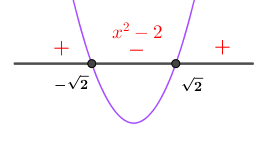
\includegraphics[width=0.4\textwidth]{imagenes/imagenes01/T01IM04.png}
			\end{figure}
				
				 *** $|x^2+3|\ge 5 \quad \to \quad x^2+3\le -5: \; x^2\le -8; \; \nexists x \qquad  \vee \qquad  x^2+3\ge 5: \; x^2\ge 2; \; x^2-2\ge 0$ De donde, procediendo como en el caso anterior para estudiar el signo de $x^2-2$ viendo previamente cuando $x^2-2=0$ y representando en $\mathbb R$ para estudiar los signos que toma $x^2-2$, usando la misma figura anterior, obtenemos como solución: $]-\infty, -\sqrt 2]\; \cup \; [\sqrt 2, \infty[$
		\end{proofw}
		
		\begin{ejre}
			Resuelve: $|x-1|+|4-2x|=4$
		\end{ejre}
		
		\begin{proofw}\renewcommand{\qedsymbol}{$\diamond$}
		
			Veamos cuando cambia el signo de los valores absolutos y representaremos en $\mathbb R$
			
			$x-1=0 \to  x=1; \qquad 4-2x=0 \to x=2$. Representamos en $\mathbb R$ los puntos $1$ y $2$ lo que nos divide el eje real en tres zonas donde analizar la ecuación como se muestra en la figura.
			
			\begin{figure}[H]
			\centering
				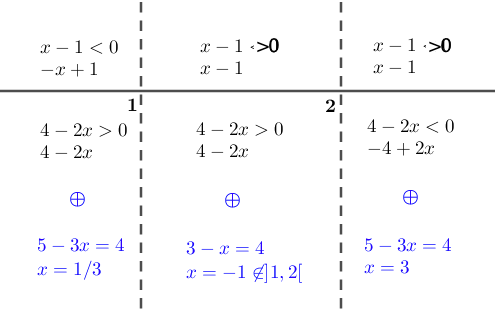
\includegraphics[width=0.85\textwidth]{imagenes/imagenes01/T01IM05.png}
			\end{figure}
			
			Soluciones:  $x=3\; $ y $\; x=1/3$.
		\end{proofw}
		
		\begin{ejre}
			Resuelve: $|x-1|\le2|x-3|$
		\end{ejre}
		
		\begin{proofw}\renewcommand{\qedsymbol}{$\diamond$}
		
			Recordemos la estrategia adoptada en la demostración del teorema 2, \emph{"para probar una desigualdad entre dos números positivos es suficiente con probar esa desigualdad para sus cuadrados"}
			
			$|x-1|\le 2|x-3| \to (x-1)^2 \le 4(x-3)^2$ Desarrollando los cuadrados y llevándolo toda a un miembro, obtenemos: $3x^2-22x+35\ge 0$.
			
			Para resolver una inecuación de segundo grado procedemos, como para resolver una inecuación de orden mayor o igual a $2$ o sobre un cociente de polinomios, buscando los ceros de la ecuación (numerador y denominador, si se trata de un cociente) y representando en el eje real donde se estudian los signos que toma el polinomio o cociente)
			$3x^2-22x+35=0 \to x=7/3 \; \vee \; x=5$. Por lo que hemos de estudiar, factorizando la expresión: $3(x-7/3)(x-5)\ge 0 \to (3x-7)(x-5)\ge 0$.
			
			En esta ocasión, vamos a resolver el problema con la ayuda de una tabla en lugar de una figura, donde estudiaremos los signos que toman los factores que forman la expresión a estudio.
			
			
			
		\begin{table}[H]
		\centering
		\begin{tabular}{|c|c|c|c|c|c|}
		\hline
	 		Intervalo & $]-\infty,7/3[$ & $7/3$ & $]7/3,5[$ & $5$ & $[5,\infty[$ \\ \hline
	 		$(3x-7)$ & $-$ & $0$ & $+$ & $+$ & $+$ \\ \hline
	 		$(x-5)$ & $+$  & $+$  & $+$ & $0$ & $-$ \\ \hline
	 		$(3x-7)(x-5)$& $-$ & $0$ & $+$ & $0$ & $-$  \\ \hline
		\end{tabular}
		\end{table}
			
		Puesto que buscábamos las zonas en que $(3x-7)(x-5)\ge 0$, la solución es: $[7/3, 5]$
			
		\end{proofw}
		
		\begin{ejre}
			Resuelve:  $\left| \dfrac {x+2}{x-6} \right| - \left| \dfrac {x-1}{x-3} \right| \le 0$ 		\end{ejre}
		
		\begin{proofw}\renewcommand{\qedsymbol}{$\diamond$}
		
			$\left| \dfrac {x+2}{x-6} \right| - \left| \dfrac {x-1}{x-3} \right| \le 0 \to \dfrac {|x+2|}{|x-6|} \le  \dfrac {|x-1|}{|x-3|} $. Como los denominadores son positivos, podemos multiplicar en cruz y el sentido de la desigualdad no varia.
			
			$|x+2|\cdot |x-3|\le |x-1| \cdot |x-6|$. Usando de nuevo la estrategia del teorema 2, 
				\emph{"para probar una desigualdad entre dos números positivos es suficiente con probar esa desigualdad para sus cuadrados"}.
			
			$(x+2)^2\cdot (x-3)^2\le (x-1)^2 \cdot(x-6)^2 \to ... \to 12x^3-72x^2+96x \le 0 $. dividiendo por 12 y factorizando (buscando ceros a la expresión), $x(x-2)(x-4)\le 0$. Veamos la tabla de signos.
			
			
	\begin{table}[H]
	\centering
	\begin{tabular}{|c|c|c|c|c|c|c|c|}
	\hline
	 Intervalos &$]-\infty, 0[$  &$0$  &$]0,2[$  &$2$ & $]2,4[$ & $4$ & $]4,\infty[$ \\ \hline
	 $x$& $-$ & 0 & + & + & + & + & + \\ \hline
 	 $x-2$& $-$ & $-$ & $-$ & 0 & + & + & + \\ \hline
 	 $x-4$& $-$ & $-$ & $-$ & $-$ & $-$ & 0 & +\\ \hline
 	 $x(x-2)(x-4)$& $-$ & 0 & + & 0 & $-$ & 0 & +\\ \hline
	\end{tabular}
	\end{table}
			
			Como nos queremos quedar con las zonas en que $x(x-2)(x-4)\le 0$, \emph{pero no podemos tomar, en ningún caso, ni el $3$ ni el $6$, que anularan los denominadores del ejercicio pedido}, la solución es:  $]-\infty, 0] \cup [2,4] \sim \{ 3 \}$



		\end{proofw}
		
		\begin{ejre}
			Resuelve $\left| \dfrac {3x+12}{x+2} \right| \ge 1$
		\end{ejre}
		
		\begin{proofw}\renewcommand{\qedsymbol}{$\diamond$}
		
			Establezcamos primero que en ningún momento podemos admitir la solución $x=-2$ puesto que anula un denominador de la inecuación de partida.
			
			$\left| \dfrac {3x+12}{x+2} \right| \ge 1 \to \dfrac {3x+12}{x+2} \le -1 \; (i)\quad \vee \quad \dfrac {3x+12}{x+2} \ge 1 \; (ii)$
			
			Resolveremos las dos inecuaciones $(i)$ e $(ii)$ por separado y tomaremos como solución la unión de las mismas, excluyendo al $-2$ si está en ellas.
 
 			Inecuación $(i): \quad \dfrac {3x+12}{x+2} \le -1 \to \dfrac {3x+12}{x+2} +1\le 0 \to \dfrac {4x+14}{x+2} \le 0$		
 			
 			Los ceros de esta expresión son $x=-7/2$ y $x=-2$ que dictarán los intervalos en que estudiar el signo del cociente. Lo vemos en la siguiente tabla:
 			
 			
 			
 			\begin{table}[H]
 			\centering
			\begin{tabular}{|c|c|c|c|c|c|}
			\hline
 			Intervalos&$]-\infty,-7/2[$  &$-7/2$  &$]-7/2,-2[$  & $-2$ &$]-2,\infty[$ \\ \hline
 			$4x+14$& $-$ & 0 & + &+  & +\\ \hline
 			$(x+2)$& $-$ & $-$  & $-$  &0  & +\\ \hline
 			$\dfrac {4x+14}{x+2}$& + & 0 & $-$ & $\nexists$ & +\\ \hline
			\end{tabular}
			\end{table}
			
			 Solución $(i):\qquad [-7/2,2[$
			
			Inecuación $(i): \quad \dfrac {3x+12}{x+2} \ge 1 \to \dfrac {3x+12}{x+2} -1\ge 0 \to \dfrac {2x+10}{x+2} \ge 0$	
			
			Los ceros de esta expresión son $x=-5$ y $x=-2$ que dictarán los intervalos en que estudiar el signo del cociente. Lo vemos en la siguiente tabla:
 			
 			
 			
 			\begin{table}[H]
 			\centering
			\begin{tabular}{|c|c|c|c|c|c|}
			\hline
 			Intervalos&$]-\infty,-5[$  &$-5$  &$]-5,-2[$  & $-2$ &$]-2,\infty[$ \\ \hline
 			$2x+10$& $-$ & 0 & + &+  & +\\ \hline
 			$(x+2)$& $-$ & $-$  & $-$  &0  & +\\ \hline
 			$\dfrac {2x+10}{x+2}$& + & 0 & $-$ & $\nexists$ & +\\ \hline
			\end{tabular}
			\end{table}
 			
 			 Solución $(i):\qquad ]-\infty,-5]\;  \cup \;  ]-2,\infty[$
 			
 			 Finalmente, la solución del problema la formarán la unión de los intervalos solución $(i)$ y $(ii)$, excluyendo, si es necesario al $\{ -2 \}$:
 			
 			 Solución:  $]-\infty, -5] \; \cup\;  [-7/2, -2[ \; \cup\;  ]-2, \infty[$
 			
		\end{proofw}
		
		
		
		\begin{ejre}
			 Resuelve: $4-|x|\le \left|\;  |2x| -6 \;   \right|$	 
		\end{ejre}
		
		\begin{proofw}\renewcommand{\qedsymbol}{$\diamond$}
				
				$4-|x|\le \left|\;  |2x| -6 \;   \right| \to 4\le \left|\;  |2x| -6 \;   \right|\; +|x|\; \to \; 4 \le 2|\;|x|-3 \; | +|x|$	
				
				\vspace{2mm} Los puntos críticos son (donde cambia el signo), en esta ocasión, 
				
				$|x|=0\to x=0; \qquad |x|-3=0 \to |x|=3 \to x=\pm 3$
				
				La siguiente tabla nos permitirá eliminar los valores absolutos en nuestra inecuación que presenta cuatro casos.
				
				
		\begin{table}[H]
		\centering
		\begin{tabular}{|c|c|c|c|c|}
		\hline
		 	Intervalos& $]-\infty, -3[$ & $[-3,0[$ & $[0,3[$ & $[3,\infty[$ \\ \hline
		 	$x$& $-$ & $-$ & + & + \\ \hline
		 	$|x|-3$& + & $-$ & $-$ & + \\ \hline
		 	casos& $i)$ & $ii)$ & $iii)$ & $iv)$ \\ \hline
		\end{tabular}
		\end{table}
			
			 $\circ$ Caso $i)\quad x\in \; ]-\infty,-3[$	
			
			$ 2|\;|x|-3 \; | +|x| \ge 4 \to 2 (\; |x|-3 \; )+(-x)\; = \; 2(-x-3)-x=-3x-6\ge 4$ 
			
			De donde: $x\le -10/3$
			
			\hspace{10mm}Sol $i):\quad ]-\infty,-10/3] \; \cap\;  ]-\infty,-3[ \; = \; ]-\infty,-10/3]$
			
			
			
			 $\circ$ Caso $ii) \quad x\in \; [-3,-0[$	
			
			$ 2|\;|x|-3 \; | +|x| \ge 4 \to 2(-\;(-x-3) \;) +(-x)=2((x+3)-x=x+6\ge 4  $
			
			De donde: $x\ge -2$
			
			\hspace{10mm}Sol $ii) \quad  [-3,0]\; \cap \; [-2,\infty[ \; = \; [-2,0[ $
			
			
			
			$\circ$ Caso $iii) \quad x\in \; [0,3[$	
			
			$ 2|\;|x|-3 \; | +|x| \ge 4 \to 2(-(x-3))+x=-x+6\ge 4 $
			
			De donde $x\le 2$
			
			\hspace{10mm} Solución $iii) \quad [0,3[ \; \cap \; ]-\infty, 2]\; = \; [0,2] $
			
			
			 $\circ$ Caso $iv) \quad x\in \; [3,\infty[$	
		
			$ 2|\;|x|-3 \; | +|x| \ge 4 \to 2(x-3)+x=3x+6\ge 4  $
			
			De donde $x\ge 10/3$
			
			\hspace{10mm} Solución $iv) \quad [3,\infty[\; \cap \; [10/3, \infty[ \; = \; [10/3, \infty[ $
			
			 Finalmente, la solución estará formada por la unión de las soluciones de los cuatro casos:
			
			\hspace{10mm} \emph{Solución final:} $]-\infty, -10/3]\; \cup \; [-2,2] \; \cup \; [10/3, \infty[$ 
			
		\end{proofw}
		
		
		\begin{ejre}
			Resuelve: $\dfrac {|x-1|-|2x+3|}{3x-4}\ge 0;\; x\neq \dfrac 4 3$
		\end{ejre}
		\begin{proofw}\renewcommand{\qedsymbol}{$\diamond$}
		
				Los puntos críticos, que hacen cambiar el signo a los argumentos del valor absoluto son, en este caso: $x-1=0 \to  x=1; \quad 2x+3=0 \to x=-3/2;\quad x\neq 4/3$ (anula el denominador).
				
				 Para resolver este problema volveremos a usar una imagen, de este modo el lector tiene dos modelos distintos de abordar el problema: en forma de tabla o de gráfico-imagen.
				
			\begin{figure}[H]
			\centering
				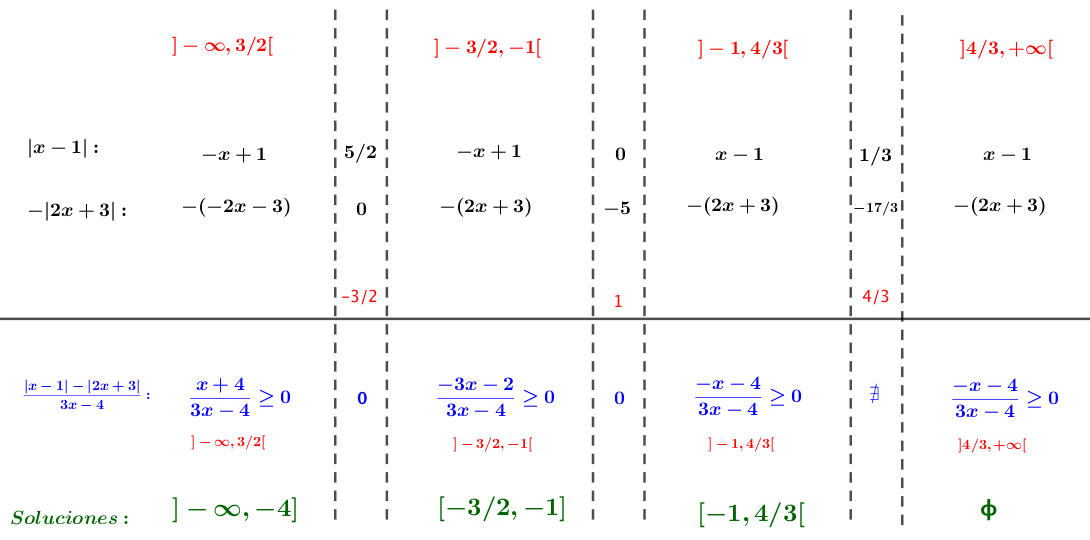
\includegraphics[width=1\textwidth]{imagenes/imagenes01/T01IM06.png}
			\end{figure}
			
			 La solución final es $\; ]-\infty, -4] \cup [-3/2,4/3[$
				
		\end{proofw}
		
	    \emph{Nota:}  $\emptyset$ es símbolo del conjunto vacío.
		
		
		
		\begin{ejre} $\divideontimes$.
			Demuestra la fórmula del \textbf{Binomio de Newton:}	
			\label{ejre:binomio-newton}
			\begin{equation}
				\forall a,b \in \mathbb R,\; \forall n \in \mathbb N: \quad (a+b)^n = \sum_{k=0}^n {\left( \begin{matrix} n \\ k \end{matrix}  \right)a^{n-k}\; b^k}
			\end{equation}
		\end{ejre}
		
		\begin{proofw}\renewcommand{\qedsymbol}{$\diamond$}
		
				Aplicaremos el \emph{Principio de inducción}: para $n=1$ la igualdad del enunciado se cumple  trivialmente.
				
				Supongamos la igualdad verdadera para $n$, entones, para $n+1$ tendremos (recordando las propiedades de los números combinatorios):
				
				\hspace{25mm}$(a+b)^{n+1}=(a+b)(a+b)^n=(a+b)\; \sum_{k=0}^n {\left( \begin{matrix} n \\ k \end{matrix}  \right)a^{n-k}\; b^k}=$
				
			    \hspace{25mm}$={\sum_{k=0}^n \left( \begin{matrix} n \\ k \end{matrix}  \right)a^{n+1-k}\; b^k}+\sum_{k=0}^n {\left( \begin{matrix} n \\ k \end{matrix}  \right)a^{n-k}\; b^{k+1}}$
				
				\hspace{25mm}$ =\sum_{k=0}^n {\left( \begin{matrix} n \\ k \end{matrix}  \right)a^{n+1-k}\; b^k}+\sum_{k=1}^{n+1} {\left( \begin{matrix} n \\ k-1 \end{matrix}  \right)a^{n+1-k}\; b^{k}} $
				
				\hspace{25mm} $ = a^{n+1}+b^{n+1}+\sum_{k=1}^n 
				\left[ \left( \begin{matrix} n \\ k \end{matrix}  \right) + \left( \begin{matrix} n \\ k-1 \end{matrix}  \right)    \right]a^{n+1-k}\; b^k=$
				
				\hspace{25mm} $=\sum_{k=0}^{n+1} {\left( \begin{matrix} n+1 \\ k \end{matrix}  \right)a^{n+1-k}\; b^k}$
				
		\end{proofw}
		
		
		
		\begin{ejre} $\divideontimes$.
			Demuestra que: $1^3+2^3+3^3+\; ...\; n^3= [n(n+1)/2]^2$
		\end{ejre}
		
		\begin{proofw}\renewcommand{\qedsymbol}{$\diamond$}
		
			Aplicamos el \emph{principio de inducción} y comprobamos, primero, que la fórmula se cumple para $n=1$, lo cual es obvio. Suponemos que se cumple para $n$ y veamos que ocurre para $n+1$
			
				 $1^3+2^3+3^3+\; ...\; n^3 \; \; +\; (n+1)^3\; =  [n(n+1)/2]^2 \; \; +(n+1)^3=$
				
				 $=  \left( \dfrac {n(n+1}{n} \right)^2 + (n+1)^3=\dfrac {(n^2+n)^2+4(n+1)^3}{4}= \frac 1 4 [n^4+6n^3+13n^2+12n+4]=$
				
				  $=\frac 1 4 [n^4+6n^3+13n^2+12n+4]=$factorizando por Ruffini: $=(n+1)^2(n+2)^2/4$
				
				=[que podemos escribir como] $=\left[ \dfrac {(n+1)(n+2)}{2} \right]^2$, que es la formula general al sustituir $n+1$ por $n$.
		\end{proofw}
		
		\begin{ejre} $\divideontimes$.
			Demostrar que no existe un número racional mínimo mayor que cero.
		\end{ejre}
		
		\begin{proofw}\renewcommand{\qedsymbol}{$\diamond$}
		
		En la demostración por reducción al absurdo se comienza por asumir lo contrario y nuestra tesis sería: existe un número racional mínimo mayor que cero: $r_0$.

		Ahora tomemos $x = r_0/2$. Por lo tanto $x$ es un número racional mayor que cero, y $x<r_0$. Eso es un absurdo, pues contradice la hipótesis de partida de que $r_0$ era el número racional mínimo. Por lo tanto se debe concluir que la proposición asumida como cierta: $``$hay un número racional mínimo mayor que cero$"$ es falsa.
		\end{proofw}
		
		\begin{ejre} $\divideontimes$.
			Demostrar que hay infinitos números primos.
		\end{ejre}
		
		\begin{proofw}\renewcommand{\qedsymbol}{$\diamond$}
		
		Existen numerosas demostraciones sobre que existen infinitos números primos, la primera de la que se tiene constancia es de Euclides, donde queda demostrado mediante 	\emph{Reductio ad absurdum} en la Proposición 20 del libro IX de Elementos (Hay más números primos que cualquier cantidad propuesta de números primos).
		
		Partiendo de suponer que lo cierto es lo contrario, por lo cual nuestra tesis quedara: $``$Los números primos son finitos$"$, entonces tenemos $n$ números primos que seran $P=p_1,\; p_2,\; ...,\; p_n$

		Entonces se toma ahora el siguiente número: $m=p_1 \cdot p_2 \cdot \; ...\cdot\; p_n+1$

		Tenemos que $m$ es el producto de todos los primos más uno, y $m$ no es un número primo, pues no se encuentra en la lista anterior, luego ha de ser un número compuesto.

 		Si dividimos $m$ por cualquiera de los primos que tenemos, todos ellos en $P$, nos da resto uno. Para que $m$ sea compuesto debería ser divisible por otro número que no está en nuestra lista de todos los números primos.
		
		Entonces llegamos a una contradicción de nuestra tesis $``$Los números primos son finitos$"$ que es falsa, por lo cual s existen infinitos números primos.
		\end{proofw}
		
		\begin{ejre} $\divideontimes$.
			Dados 5 puntos cualesquiera dentro de un triángulo equilátero de lado 2, al menos dos de ellos están a una distancia, el uno del otro, menor que 1.
		\end{ejre}
		
		\begin{proofw}\renewcommand{\qedsymbol}{$\diamond$}
		
			Está claro que por estar dentro de un triángulo equilátero de lado 2, cualesquiera dos puntos, de los cinco que hemos elegido, están a una distancia menor que 2, pero ?`podemos afirmar que siempre habrá dos de ellos que están a una distancia menor que 1?

			Para aplicar el principio del palomar se consideran los puntos medios de los lados del triángulo y se unen con segmentos, lo cual divide al triángulo en cuatro triangulitos equiláteros de lado 1. Como son cuatro triángulos de lado 1 (que serán nuestros palomares) y cinco puntos (que serán nuestras palomas), entonces habrá dos puntos en el mismo triángulo equilátero de lado 1, y esos dos están a una distancia menor que 1.
			
			\begin{figure}[H]
			\centering
				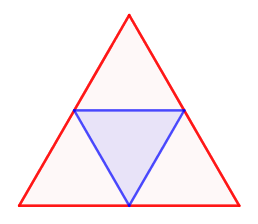
\includegraphics[width=0.3\textwidth]{imagenes/imagenes01/T01IM07.png}
			\end{figure}
		\end{proofw}
		
		%\clearpage.   corte de página
		
	
	\subsection{Ejercicios Propuestos}
	
		
		\begin{enumerate}[1).-  ]
		\item $4x+1<2x \qquad \qquad$ 
		
		\rightline{\textcolor{gris}{Solución: $]-\infty, -1/2[$}}
	
		\item $2x-1\ge0$
		 
		\rightline{\textcolor{gris}{Solución: $[1/2,\infty[$}}
		
		\item $\dfrac {2x+1}{x+3}>3$
		
		\rightline{\textcolor{gris}{Solución: $]-8,-3[$}}
	
		\item $x^3-3x^2-10x+24<0$
		
		\rightline{\textcolor{gris}{Solución: $]-\infty, -3[ \cup ]2,4[$}}
		
		\item $|x+2|\ge 5$
		
		\rightline{\textcolor{gris}{Solución: $]-\infty, -7] \cup [3,\infty[$}}
		
		\item $ \left| \dfrac 2 x -3 \right| \le 5$
		
		\rightline{\textcolor{gris}{Solución: $]-\infty,-1]\cup [1/4, \infty[$}}
		
		
		\item $ \left| \dfrac {2x-1} x \right| > 2$
			
		\rightline{\textcolor{gris}{Solución: $ ]-\infty, 0[\cup]0,1/4[ $}}
		
		\item $|x|+|x+1|=2$
		
		\rightline{\textcolor{gris}{Solución: $\{ -3/2;\; 1/2 \}$}}
		
		\item $|x-2|^2-5|x-2|+6=0$
		
		\rightline{\textcolor{gris}{Solución: $\{ -1, 0, 4, 5  \}$}}
		
		\item $|x-2|-|x+2|=|x|$
		 
		\rightline{\textcolor{gris}{Solución: $ \{ -4,0 \}$}}
		
		\item $|x^2+3x|=|x+3|$
		
		\rightline{\textcolor{gris}{Solución: $\{ -3, -1, 1 \} $}}
		
		\item $\dfrac {|x^2-16|}{x+4}\le \dfrac {x^2}{|x-1|}$
		
		\rightline{\textcolor{gris}{Solución: $ ]-\infty, -4[ \cup [4/5, 1[\cup ]1, \infty[  $}}
		
		\item $ \left|\dfrac {3|x|-x}{x+1} \right| < \dfrac 1 {x+1}$
		
		\rightline{\textcolor{gris}{Solución: $ ]-1/4, 1/2[$}}
		
		
		\end{enumerate}

		
		
	$\divideontimes$ AMPLIACIÓN: Aplicaciones \emph{curiosas}. \label{curiosidades1}
		
		\begin{multicols}{2}
			
		
		$\sqrt{12+\sqrt{12+\sqrt{12+...}}}=x$  
		
		
		$x^{x^{x^{...}}}=2$
		
		
		$\sqrt {x \sqrt {x \sqrt {x \sqrt {...}}}}=?$
		
		$7-\dfrac {12}{7-\dfrac {12}{7-\dfrac {12}{7-\dfrac {7}{12- ...}}}}=x$
		
		$\dfrac {1}{1+2\cdot \left( \dfrac {1}{1+2\cdot \left( \dfrac {1}{1+ ...} \right)} \right)}=x$
		
		$\sqrt{5+\sqrt{5-\sqrt{5+\sqrt{5- ...}}}}=\dfrac {a+\sqrt{b}}{c} \to \mbox{calcula: } a^2+b^2+c^2$
		
		\end{multicols}
		
		
		\textcolor{gris} {Resolvemos uno de estos problemas, p.e.:}
		
		\textcolor{gris} {$\dfrac {1}{1+2\cdot \left( \dfrac {1}{1+2\cdot \left( \dfrac {1}{1+ ...} \right)} \right)}=x \to x=\dfrac {1}{1+2[x]} \to x+2x^2=1;\; 2x^2+x-1=0$}
		
		\textcolor{gris} {$\to x=1 \vee x=-2 \mbox{ (sin sentido)}$ }


\vspace{4mm}

\textit{para la redacción de este capítulo me ha sido de gran ayuda los apuntes de catedrático de apuntes del catedrático F.J. Pérez Gonzalez, catedrático del departamento de Análisis Matemático de la Universidad de Granada. Muchas gracias por compartir tu saber.}

